\section{Pivotal configurations.}
Let $T$ be a dipolar tree.
Label the poles of $T$ by $p_1$ and $p_2$ and the reaming vertexes by $x_1,x_2,\dots,x_n$.

Assume $A$ is a $\CBB[0]$ complete length space.

A point array $p_1,p_2,x_1,\dots x_n\in A$ together with choice one geodesic connecting adjacent vertexes of $T$ will be called \emph{geodesic $T$-tree};
it contains one geodesic $[p_1,p_2]$ and $n$ geodesics  $[p_i,x_j]$.

A point array $\~p_1$, $\~p_2$, $\~x_1,\dots\~x_n\in \HH$ will be called \emph{pivotal configuration} of the geodesic $T$-tree in $A$
if 
\begin{enumerate}[(i)]
\item $|\~p_1-\~p_2|= |p_1-p_2|$,
\item $|\~p_i-\~x_j|= |p_i-p_j|$ for any edge $(p_i,x_j)$ in $T$ and
\item $\measuredangle[\~p_j\,^{\~x_k}_{\~p_i}]_{\HH}=\measuredangle[\~p_j\,^{\~x_k}_{\~p_i}]_A$
for any hinge  $[p_j\,^{x_k}_{\~p_i}]$ in $T$.
\end{enumerate}

Note that by angle comparison 
\[|\~x_i-\~p_j|_{\RR^n}\ge |x_i-p_j|_A\]
for any $i$ and $j$.
Therefore, in order to check that a pivotal configuration $\~p_1$, $\~p_2$, $\~x_1,\dots\~x_n\in \RR^n$ satisfies the conditions in the $T$-tree comparison (see Section~\ref{sec:intro}) it is sufficient to check that 
\[|\~x_i-\~x_j|_{\RR^n}\ge |x_i-x_j|_A\]
for all $i,j$.

\begin{thm}{Rigidity lemma}\label{lem:rigidity}
Let $A$ be a $\CBB[0]$ complete length space.
Suppose  $\~p_1$, $\~p_2$, $\~x_1,\dots\~x_n\in \HH$ is a pivotal configuration for a geodesic tree  with the vertexes $p_1,p_2,x_1,\dots x_n\in A$.
Assume that
\[|\~x_i-\~x_j|_\HH\le |x_i-x_j|_A 
\eqlbl{eq:pivotal-comparison}\]
for any pair $(i,j)$ and the convex hull $\~K$ of $\{\~x_1,\dots\~x_n\}$ intersects the line $\~p_1\~p_2$.
Then, for arbitrary pair $(i,j)$, the equality holds in \ref{eq:pivotal-comparison} .
\end{thm}

\parit{Proof.}
Given a point $\~z$ on the line $p_1p_2$,
let us construct a point $z\in A$.

If $\~z\in [p_1,p_2]$ then set $z\in [p_1,p_2]$ to be the corresponding point;
that is $|z-p_i|=|~z-\~p_i|$ for $i=1,2$.

In the remaining case, $\~z\notin [\~p_1,\~p_2]$, without loss of generality, we can assume that $\~z$ lies on the half line starting at $\~p_1$.
In this case set $z$ to be the image of $p_2$ for the $(\tfrac12\cdot \dist_{p_1}^2)$-gradient flow of $p_2$ for time $t=\ln \tfrac{|\~z-\~p_1|}{|\~p_2-\~p_1|}$.
In both cases the comparsison implies 
\begin{align*}
|x_i-z|_A &\le |\~x_i-\~z|_{\RR^2},
&
|x_j-z|_A &\le |\~x_j-\~z|_{\RR^2}.
\end{align*}
It remains to apply Kirszbraun rigidity theorem.
\qeds


Up to a motion of $\HH^n$, a pivotal configuration is completely described by the angles $\alpha_{i,j}$ between the half-planes passing $\~x_i$ and $\~x_j$ with $\~p_1 \~p_2$ as the the boundary line.

Let us denote by $\beta_{i,j}$ the minimal angle between the halfplanes $\~p_1 \~p_2 \~x_i$ and $p_1p_2 x_j$ in a pivotal configuration such that $|\~x_i-\~x_j|_{\RR^3}\ge|\~x_i-\~x_j|_A$. 
Note that a pivotal  configuration $\~p_1,\~p_2,\~x_1,\dots,\~x_n$ satisfies the conditions in the definition of comparison if and only if $\alpha_{i,j}\ge \beta_{i,j}$ for all pairs $(i,j)$.

As a corollaries of the rigidity lemma, we get the following.

\begin{thm}{Corollary}\label{cor:|x-x|}
For any geodesic dipolar tree  in a complete $\CBB[0]$ length space the following conditions hold:
\begin{enumerate}[(a)]
\item For any pair $i$ and $j$, we have
\[\beta_{i,j}\le \pi.\]
\item For any triple $i$, $j$ and $k$,  we have
\[\beta_{i,j}+\beta_{j,k}+\beta_{k,i}\le 2\cdot\pi.\]
\end{enumerate}
In other words, 
\begin{enumerate}[(a)]
\item For any broken geodesic line $x_1p_1p_2x_2$ in a nonnegatively curved Alexandrov space $A$ there is a pivotal configuaration $\~p_1,\~p_2,\~x_1,\~x_2\in \RR^2$ such that 
\[|\~x_1-\~x_2|_{\RR^2}\ge |x_1-x_2|_A.\]
\item For any geodesic (2-1)-tree $x_1x_2p_1p_2x_3$ in a nonnegatively curved Alexandrov space $A$ there is a pivotal configuaration $\~p_1,\~p_2,\~x_1,\~x_2,x_3\in \RR^3$ such that 
\begin{align*}
|\~x_1-\~x_2|_{\RR^2}&\ge |x_1-x_2|_A,
\\
|\~x_2-\~x_3|_{\RR^2}&\ge |x_2-x_3|_A,
\\
|\~x_3-\~x_1|_{\RR^2}&\ge |x_3-x_1|_A.
\end{align*}
\end{enumerate}

\end{thm}

\section{Six point comparison}


\begin{thm}{Theorem}
Any Alexandrov space with nonnegative curvature satisfies the tree comparison for the following two trees:

\begin{comment}
\begin{center}
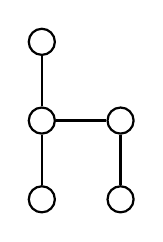
\begin{tikzpicture}[scale=1,
  thick,main node/.style={circle,draw,font=\sffamily\bfseries,minimum size=3mm}]
  \node[main node] (1) at (0,0) {};
  \node[main node] (2) at (0,1){};
  \node[main node] (3) at (0,2){};
  \node[main node] (4) at (1,0) {};
  \node[main node] (5) at (1,1) {};
  

  \path[every node/.style={font=\sffamily\small}]
   (1) edge node[above]{}(2)
   (2) edge node[above]{}(3)
   (2) edge node[above]{}(5)
   (4) edge node[above]{}(5);
\end{tikzpicture}
\hskip10mm
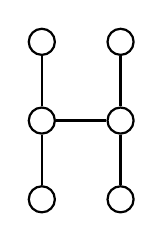
\begin{tikzpicture}[scale=1,
  thick,main node/.style={circle,draw,font=\sffamily\bfseries,minimum size=3mm}]

  \node[main node] (1) at (0,0) {};
  \node[main node] (2) at (0,1){};
  \node[main node] (3) at (0,2){};
  \node[main node] (4) at (1,0) {};
  \node[main node] (5) at (1,1) {};
  \node[main node] (6) at (1,2) {};

  \path[every node/.style={font=\sffamily\small}]
   (1) edge node[above]{}(2)
   (2) edge node[above]{}(3)
   (2) edge node[above]{}(5)
   (4) edge node[above]{}(5)
   (5) edge node[above]{}(6);
\end{tikzpicture}
\hskip10mm
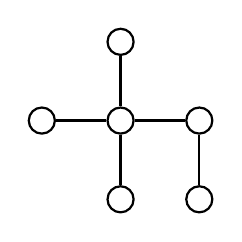
\begin{tikzpicture}[scale=1,
  thick,main node/.style={circle,draw,font=\sffamily\bfseries,minimum size=3mm}]

  \node[main node] (1) at (0,1) {};
  \node[main node] (2) at (1,0){};
  \node[main node] (3) at (1,1){};
  \node[main node] (4) at (1,2) {};
  \node[main node] (5) at (2,0) {};
  \node[main node] (6) at (2,1) {};

  \path[every node/.style={font=\sffamily\small}]
   (1) edge node[above]{}(3)
   (2) edge node[above]{}(3)
   (3) edge node[above]{}(6)
   (4) edge node[above]{}(3)
   (5) edge node[above]{}(6);
\end{tikzpicture}
\end{center}
\end{comment}

\end{thm}


\parit{Proof.} 
Fix a bipolar geodesic tree with the poles $p_1$, $p_2$ and the remaining vertexes $x_1,x_2, x_3,x_4$.
Define the values $\{\beta_{i,j}\}$ for each pair $i,j$ as in the previous section.

Let us list the values $\{\beta_{i,j}\}$ in the non-increasing order.
The following 6 step algorithm, we will produce a metric graph with the vertexes $x_1,x_2, x_3,x_4$.
\begin{enumerate}[1.]
\item If $\beta_{i,j}$ the first value in the list, connect vertexes $x_i$ and $x_j$ by an edge of length $\beta_{i,j}$.
\item Do the same for the second value  in the list.
\item Starting from the third step, we attach a new edge corresponding to the next value $\beta_{i,j}$ only if the already constructed edges in the graph will remain to be the shortest path between their vertexes; otherwise go to the next value in the list. 
\end{enumerate}
Denote the obtained metric graph by $\Gamma$;
note that $\Gamma$ is connected. 
If the triangle inequalities 
\[\beta_{i,k}\le \beta_{i,j}+\beta_{j,k}\]
hold for all $i,j,k$ then $\Gamma$ is the complete graph with 4 vertexes;
otherwise it will be one of the following graphs.

\begin{comment}
\begin{center}
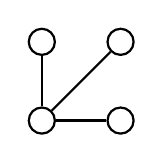
\begin{tikzpicture}[scale=1,
  thick,main node/.style={circle,draw,font=\sffamily\bfseries,minimum size=3mm}]

  \node[main node] (1) at (0,0) {};
  \node[main node] (2) at (0,1){};
  \node[main node] (3) at (1,1){};
  \node[main node] (4) at (1,0) {};

  \path[every node/.style={font=\sffamily\small}]
   (1) edge node[above]{}(2)
   (1) edge node[above]{}(3)
   (1) edge node[above]{}(4);
   
\end{tikzpicture}
\hskip10mm
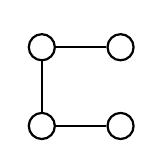
\begin{tikzpicture}[scale=1,
  thick,main node/.style={circle,draw,font=\sffamily\bfseries,minimum size=3mm}]

  \node[main node] (1) at (0,0) {};
  \node[main node] (2) at (0,1){};
  \node[main node] (3) at (1,1){};
  \node[main node] (4) at (1,0) {};

  \path[every node/.style={font=\sffamily\small}]
   (1) edge node[above]{}(2)
   (2) edge node[above]{}(3)
   (1) edge node[above]{}(4);
\end{tikzpicture}
\hskip10mm
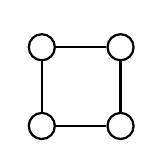
\begin{tikzpicture}[scale=1,
  thick,main node/.style={circle,draw,font=\sffamily\bfseries,minimum size=3mm}]

  \node[main node] (1) at (0,0) {};
  \node[main node] (2) at (0,1){};
  \node[main node] (3) at (1,1){};
  \node[main node] (4) at (1,0) {};

  \path[every node/.style={font=\sffamily\small}]
   (1) edge node[above]{}(2)
   (2) edge node[above]{}(3)
   (3) edge node[above]{}(4)
   (1) edge node[above]{}(4);
\end{tikzpicture}
\hskip10mm
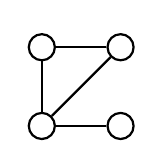
\begin{tikzpicture}[scale=1,
  thick,main node/.style={circle,draw,font=\sffamily\bfseries,minimum size=3mm}]

  \node[main node] (1) at (0,0) {};
  \node[main node] (2) at (0,1){};
  \node[main node] (3) at (1,1){};
  \node[main node] (4) at (1,0) {};

  \path[every node/.style={font=\sffamily\small}]
   (1) edge node[above]{}(2)
   (2) edge node[above]{}(3)
   (3) edge node[above]{}(1)
   (1) edge node[above]{}(4);
\end{tikzpicture}
\hskip10mm
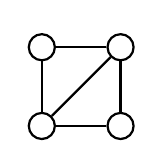
\begin{tikzpicture}[scale=1,
  thick,main node/.style={circle,draw,font=\sffamily\bfseries,minimum size=3mm}]

  \node[main node] (1) at (0,0) {};
  \node[main node] (2) at (0,1){};
  \node[main node] (3) at (1,1){};
  \node[main node] (4) at (1,0) {};

  \path[every node/.style={font=\sffamily\small}]
   (1) edge node[above]{}(2)
   (2) edge node[above]{}(3)
   (3) edge node[above]{}(1)
   (3) edge node[above]{}(4)
   (1) edge node[above]{}(4);
\end{tikzpicture}
\end{center}
\end{comment}

In the latter case, by Corollary~\ref{cor:|x-x|}, there is a geodesic graph $\~\Gamma$ in $\SS^2$ isometric to $\Gamma$.
Let $\~p_1$, $\~p_2$, $\~x_1$, $\~x_2$, $\~x_3$, $\~x_4\in \HH$ be the corresponding pivotal configuration;
denote by $\alpha_{i,j}$ the angles between the half-planes $p_1p_2x_i$ and $p_1p_2x_j$ as above.

Note that in this case
\[\alpha_{i,j}\ge \beta_{i,j}\]
for any pair $(i,j)$.
Indeed, if $x_i$ is adjacent to $x_j$ in $\Gamma$ then we have the equality holds;
otherwise the inequality follows from the triangle inequality in $\SS^2$.

\begin{comment}
\begin{wrapfigure}{r}{14 mm}
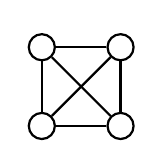
\begin{tikzpicture}[scale=1,
  thick,main node/.style={circle,draw,font=\sffamily\bfseries,minimum size=3mm}]

  \node[main node] (1) at (0,0) {};
  \node[main node] (2) at (0,1){};
  \node[main node] (3) at (1,1){};
  \node[main node] (4) at (1,0) {};

  \path[every node/.style={font=\sffamily\small}]
   (1) edge node[above]{}(2)
   (2) edge node[above]{}(3)
   (2) edge node[above]{}(4)
   (3) edge node[above]{}(1)
   (3) edge node[above]{}(4)
   (1) edge node[above]{}(4);
\end{tikzpicture}
\end{wrapfigure}
\end{comment}

It remains to consider the case when $\Gamma$ is the complete graph (see the diagram). 
In this case, let us remove the edge $(x_3,x_4)$ from $\Gamma$;
denote the obtained graph by $\Gamma'$.
Note that there is geodesic graph $\~\Gamma'$ in $\SS^2$ which is isometric to $\Gamma'$;
denote by $\~\xi_1,\~\xi_2,\~\xi_3,\~\xi_4$ the corresponding vertexes in $\~\Gamma'$.
We can (and will) assume that the vertexes $\~\xi_3$ and $\~\xi_4$ lie on the opposite side from the equator containing $[\~\xi_1,\~\xi_2]$.
Let $\~p_1$, $\~p_2$, $\~x_1$, $\~x_2$, $\~x_3$, $\~x_4\in \HH$ be the corresponding pivotal configuration;
that is, $\~\xi_i$ is the normal direction of the half-plane $\~p_1\~p_2\~x_i$ to the line $\~p_1\~p_2$.


Denote by $\~K$ the convex hull of $\~x_1,\~x_2,\~x_3,\~x_4$.

Assume the interior of $\~K$ intersects the line $\~p_1\~p_2$;
or equivalently $\~K'=\SS^2$, where $\~K'$ is the convex hull  of $\~\xi_1,\~\xi_2,\~\xi_3,\~\xi_4$.
Then by the rigidity lemma, whe have 
\[|\~x_i-\~x_j|_\HH=|x_i-x_j|_A\]
for each pair $(i,j)$.
In particular, the array $\~p_1$, $\~p_2$, $\~x_1$, $\~x_2$, $\~x_3$, $\~x_4\in \HH$ satisfies the tree comparison.

In the remaining case $\~K'\ne \SS^2$, the boundary $\partial_{\SS^2}\~K'$ is nonempty; moreover it contains at least 3 of the vertexes $\~\xi_1,\~\xi_2,\~\xi_3,\~\xi_4$.
Without loss of generality we may assume that $\~\xi_1\in \partial_{\SS^2}K$.
Denote by $\~\xi_4'$ the point on the extension of $[\~\xi_3,\~\xi_1]$ behind $\~\xi_1$ such that $|\~\xi_1-\~\xi_4'|_{\SS^2}=|\~\xi_1-\~\xi_4|_{\SS^2}$.
Since the increasing of angle increase the opposite side, we have
\begin{align*}
|\~\xi_2-\~\xi_4'|_{\SS^2}&=|\~\xi_2-\~\xi_4|_{\SS^2}=\beta_{2,4}.
\end{align*}
Note that 
\[
|\~\xi_3-\~\xi_4'|_{\SS^2}=\min\{\,\beta_{1,3}+\beta_{1,4},\,\pi-(\beta_{1,3}+\beta_{1,4})\,\} 
\]
Since $\Gamma$ is complete, we have 
\[\beta_{1,3}+\beta_{1,4}\ge \beta_{3,4}\]
and by Corollary~\ref{cor:|x-x|},
\[\beta_{1,3}+\beta_{1,4}+\beta_{3,4}\le 2\cdot\pi.\]
Therefore 
\[
|\~\xi_3-\~\xi_4'|_{\SS^2}\ge \beta_{3,4};
\]
that is, the corresponding pivotal configurations satisfies the definition of tree comparison.
\qeds



